\documentclass[11pt]{article}

\usepackage[a4paper,margin=1in]{geometry}
\usepackage{graphicx}
\usepackage{amsmath}
\usepackage{amssymb}
\usepackage{booktabs}
\usepackage{array}
\usepackage{float}
\usepackage{hyperref}
\usepackage{enumitem}
\usepackage{setspace}
\usepackage{titlesec}
\usepackage{xcolor}

\newcommand{\figref}[1]{\figurename~\ref{#1}}
\newcommand{\tabref}[1]{\tablename~\ref{#1}}
\newcommand{\secref}[1]{Section~\ref{#1}}

\usepackage{xspace}
\newcommand{\ivttriplet}{\texttt{$\langle$instrument, verb, target$\rangle$}\xspace}
\newcommand{\vtpair}{\texttt{$\langle$verb, target$\rangle$}\xspace}
\newcommand{\ivpair}{\texttt{$\langle$instrument, verb$\rangle$}\xspace}
\newcommand{\itpair}{\texttt{$\langle$instrument, target$\rangle$}\xspace}
\newcommand{\triplet}[3]{\texttt{$\langle$#1, #2, #3$\rangle$}\xspace}
\newcommand{\pair}[2]{\texttt{$\langle$#1, #2$\rangle$}\xspace}
\newcommand{\singlet}[1]{\texttt{$\langle$#1$\rangle$}\xspace}
\newcommand{\apivt}{\texttt{$AP_{IVT}$}\xspace}

\newcommand{\anatprior}{weak anatomy\xspace}
\newcommand{\Anatprior}{Weak anatomy\xspace}
\newcommand{\AnatPrior}{Weak Anatomy\xspace}

\hypersetup{
    colorlinks=true,
    linkcolor=blue,
    urlcolor=blue,
    citecolor=blue
}

\setstretch{1.08}

\title{Multimodal Large Language Models for Interaction Prediction in Two-Stage Surgical Triplet Segmentation}

\author{Oluwatosin Alabi}
\date{}

\newcommand{\todo}[1]{\textcolor{red}{\textbf{TODO: #1}}}

\begin{document}

\maketitle

\begin{abstract} 
Surgical triplet segmentation aims to jointly localise surgical instrument instances and identify the corresponding \ivttriplet interaction performed by each instrument. Although recent end-to-end architectures have demonstrated promising performance, accurate interaction prediction remains a major challenge, suggesting that dense localisation and semantic interaction understanding may benefit from being addressed separately.

In this work, we investigate multimodal large language models (MLLMs) as the multimodal interaction reasoning stage of a two-stage surgical triplet segmentation framework. Given pre-localised instrument instances, we establish a direct supervised fine-tuning baseline and evaluate several adaptation strategies, including temporal visual context, sequential dialogue prediction, distilled reasoning supervision, anatomical context priors, ontology-guided Prompting, and alternative optimisation settings.

Experiments on the CholecTripletSeg benchmark show that direct supervised fine-tuning provides a strong baseline, achieving performance comparable to specialised end-to-end triplet segmentation architectures. Among the investigated adaptations, short-range temporal context and sequential dialogue prediction provide the most consistent improvements, whereas longer temporal windows, distilled reasoning supervision, anatomical context priors, and ontology-guided Prompting do not consistently improve performance. We further show that optimisation choices, including training duration, batch size, and learning rate, can influence performance as much as changes to the modelling strategy itself.

These findings demonstrate that multimodal large language models provide an effective multimodal interaction reasoning stage within a two-stage surgical triplet segmentation framework. They further highlight the importance of careful task formulation and model optimisation. We hope this work provides practical guidance for adapting foundation models to structured surgical scene understanding tasks.
\end{abstract}

\section{Introduction}
Understanding surgical scenes is a fundamental challenge in computer-assisted intervention. Beyond detecting surgical instruments or recognising procedural phases, comprehensive scene understanding requires identifying how individual instruments interact with anatomical structures throughout an operation. Such fine-grained understanding has applications in surgical workflow analysis, skill assessment, autonomous assistance and context-aware decision support.

Surgical action triplets have emerged as an effective representation for modelling these interactions. Each interaction is represented as an \ivttriplet\ tuple describing which instrument performs which action on which anatomical structure. While early approaches predicted a single interaction label for an entire frame, recent work has shifted towards \emph{grounded} interaction understanding, where every visible instrument instance is associated with its own interaction. CholecTripletSeg extended this formulation by combining instance segmentation annotations with surgical triplet labels, enabling the study of instance-grounded triplets also known as surgical triplet segmentation.

Although recent methods have demonstrated encouraging progress, surgical triplet segmentation remains a challenging problem. Instrument localisation has reached relatively high performance, whereas verb and, in particular, target prediction remain substantially more difficult. Existing approaches typically address localisation and interaction prediction jointly within a single architecture, requiring the same model to solve both dense pixel-level segmentation and fine-grained semantic interaction prediction simultaneously.

This observation motivates a two-stage formulation of the problem. Instrument localisation and multimodal interaction reasoning require fundamentally different capabilities. The first is a dense prediction task that benefits from specialised segmentation architectures, while the second requires interpreting the relationship between an already-localised instrument and the surrounding anatomy. Rather than requiring a single model to solve both problems simultaneously, we investigate whether multimodal interaction reasoning can be performed independently once instrument instances have been grounded.

Multimodal large language models (MLLMs) have recently demonstrated remarkable capabilities in visual understanding and image-language reasoning. Although they are not designed for precise pixel-level segmentation, they are well suited to interpreting visual context and producing structured outputs, making them a promising candidate for multimodal interaction reasoning within a two-stage framework.

In this work, we investigate the use of multimodal large language models as the interaction prediction stage of a two-stage surgical triplet segmentation pipeline. Given grounded instrument instances, we first establish a direct supervised fine-tuning baseline before exploring several extensions, including temporal visual context, sequential dialoguie, distilled reasoning supervision, anatomical context priors, ontology-guided Prompting and alternative optimisation strategies. Rather than proposing a new multimodal architecture, our goal is to understand which design choices improve interaction prediction within this formulation.

Our experiments demonstrate that direct supervised fine-tuning provides a strong baseline, achieving performance comparable to specialised end-to-end triplet segmentation models. We further show that incorporating short-range temporal information and decomposing the prediction task can improve complete triplet recognition, whereas several more sophisticated additions, including distilled reasoning supervision, anatomical context priors and ontology-guided Prompting, do not consistently improve performance. Finally, our results highlight that optimisation choices can be as influential as architectural modifications when adapting multimodal large language models to surgical interaction prediction.

The main contributions of this work are:
\begin{itemize}
    \item We formulate interaction prediction as a multimodal interaction reasoning problem and investigate multimodal large language models as the reasoning stage within a two-stage surgical triplet segmentation framework.
    
    \item We establish a direct supervised fine-tuning baseline for grounded surgical interaction prediction and evaluate several extensions, including temporal context, sequential dialogue prediction, reasoning supervision, anatomical priors and ontology-guided Prompting.
    
    \item We demonstrate that short-range temporal context and sequential dialogue prediction improve interaction prediction, while several more complex reasoning-based adaptations do not consistently provide additional gains.
    
    \item We provide practical insights into adapting multimodal foundation models for fine-grained surgical interaction prediction.
\end{itemize}

\section{Related Work}

\subsection{Surgical Triplet Recognition}

Surgical action triplets, represented as \ivttriplet tuples, have become a standard representation for modelling instrument-tissue interactions in minimally invasive surgery. CholecT50 \cite{nwoye2022rendezvous} first established surgical triplet recognition as a frame-level multi-label classification task. Early methods, including TripNet~\cite{nwoye2020recognition}, focused on recognising triplets from entire images without explicitly identifying the responsible instrument. Rendezvous (RDV)~\cite{nwoye2022rendezvous} later introduced an attention-based architecture that models relationships between instruments, verbs and targets using weak localisation cues derived from class activation maps (CAMs), establishing a strong baseline for surgical triplet recognition.

Subsequent work explored a range of improvements, including temporal modelling, transformer-based architectures, self-distillation and multi-task optimisation. Representative examples include MT4MTL-KD~\cite{gui2023mt4mtl}, TERL~\cite{gui2024tail}, and more recently MEJO~\cite{zhang2025mejo}, which investigated improved optimisation and representation learning for the triplet recognition task. Despite these advances, anatomical target prediction remains substantially more challenging than instrument or verb recognition.

More recently, grounded formulations have extended triplet recognition by explicitly associating each interaction with an individual instrument instance. CholecTripletSeg ~\cite{alabi2026grounding} established the task of triplet segmentation by combining instrument instance segmentation with triplet recognition, while TargetFusionNet~\cite{alabi2026grounding} demonstrated that incorporating weak anatomical priors can improve target prediction by integrating coarse anatomical context into a Mask2Former-based architecture. Nevertheless, interaction prediction, particularly anatomical target recognition, remains the principal bottleneck.

\subsection{Multimodal Large Language Models for Surgical Understanding}
Multimodal large language models (MLLMs) have recently attracted considerable attention in surgical artificial intelligence owing to their ability to combine visual understanding with language reasoning. Early surgical MLLMs primarily focused on general vision-language tasks such as visual question answering, report generation, scene interpretation and educational assistants. For example, SurgicalGPT~\cite{seenivasan2023surgicalgpt} extends GPT-2~\cite{radford2019language} with visual tokens for surgical visual question answering, while Surgical-LLaVA~\cite{jin2024surgical} adapts instruction-tuned vision-language models for conversational understanding of surgical images and videos. These approaches demonstrate strong general reasoning capabilities but are primarily designed for open-ended vision-language understanding rather than structured surgical interaction prediction.

More recently, MLLMs have begun to be explored for surgical triplet recognition. MEJO~\cite{zhang2025mejo} incorporates MLLM-generated semantic descriptions as auxiliary prompts to enrich feature representations within a conventional multi-task triplet recognition framework while retaining a discriminative prediction architecture.

In contrast, we investigate multimodal interaction reasoning under a two-stage formulation. Given grounded instrument instances from a dedicated segmentation model, we study whether an MLLM can directly predict surgical \ivttriplet\ interactions within a two-stage triplet segmentation framework.


\section{Method}
We investigate multimodal large language models (MLLMs) as the interaction reasoning stage of a two-stage surgical triplet segmentation framework. This section describes the proposed framework, formulates the interaction reasoning problem, and presents the investigated adaptations.

Given a laparoscopic image, instrument instances are first localised using an instance segmentation model. The original image together with the grounded instrument instances are then provided to an MLLM, which predicts one verb--target interaction for every instrument instance. The complete \ivttriplet\ is obtained by combining the predicted interaction with the known instrument identity.

Unlike previous end-to-end approaches, grounding and interaction reasoning are treated as separate stages. This allows the interaction reasoning model to remain independent of the underlying segmentation architecture and enables improvements to either stage without modifying the other.

\begin{figure}[htb!]
    \centering
    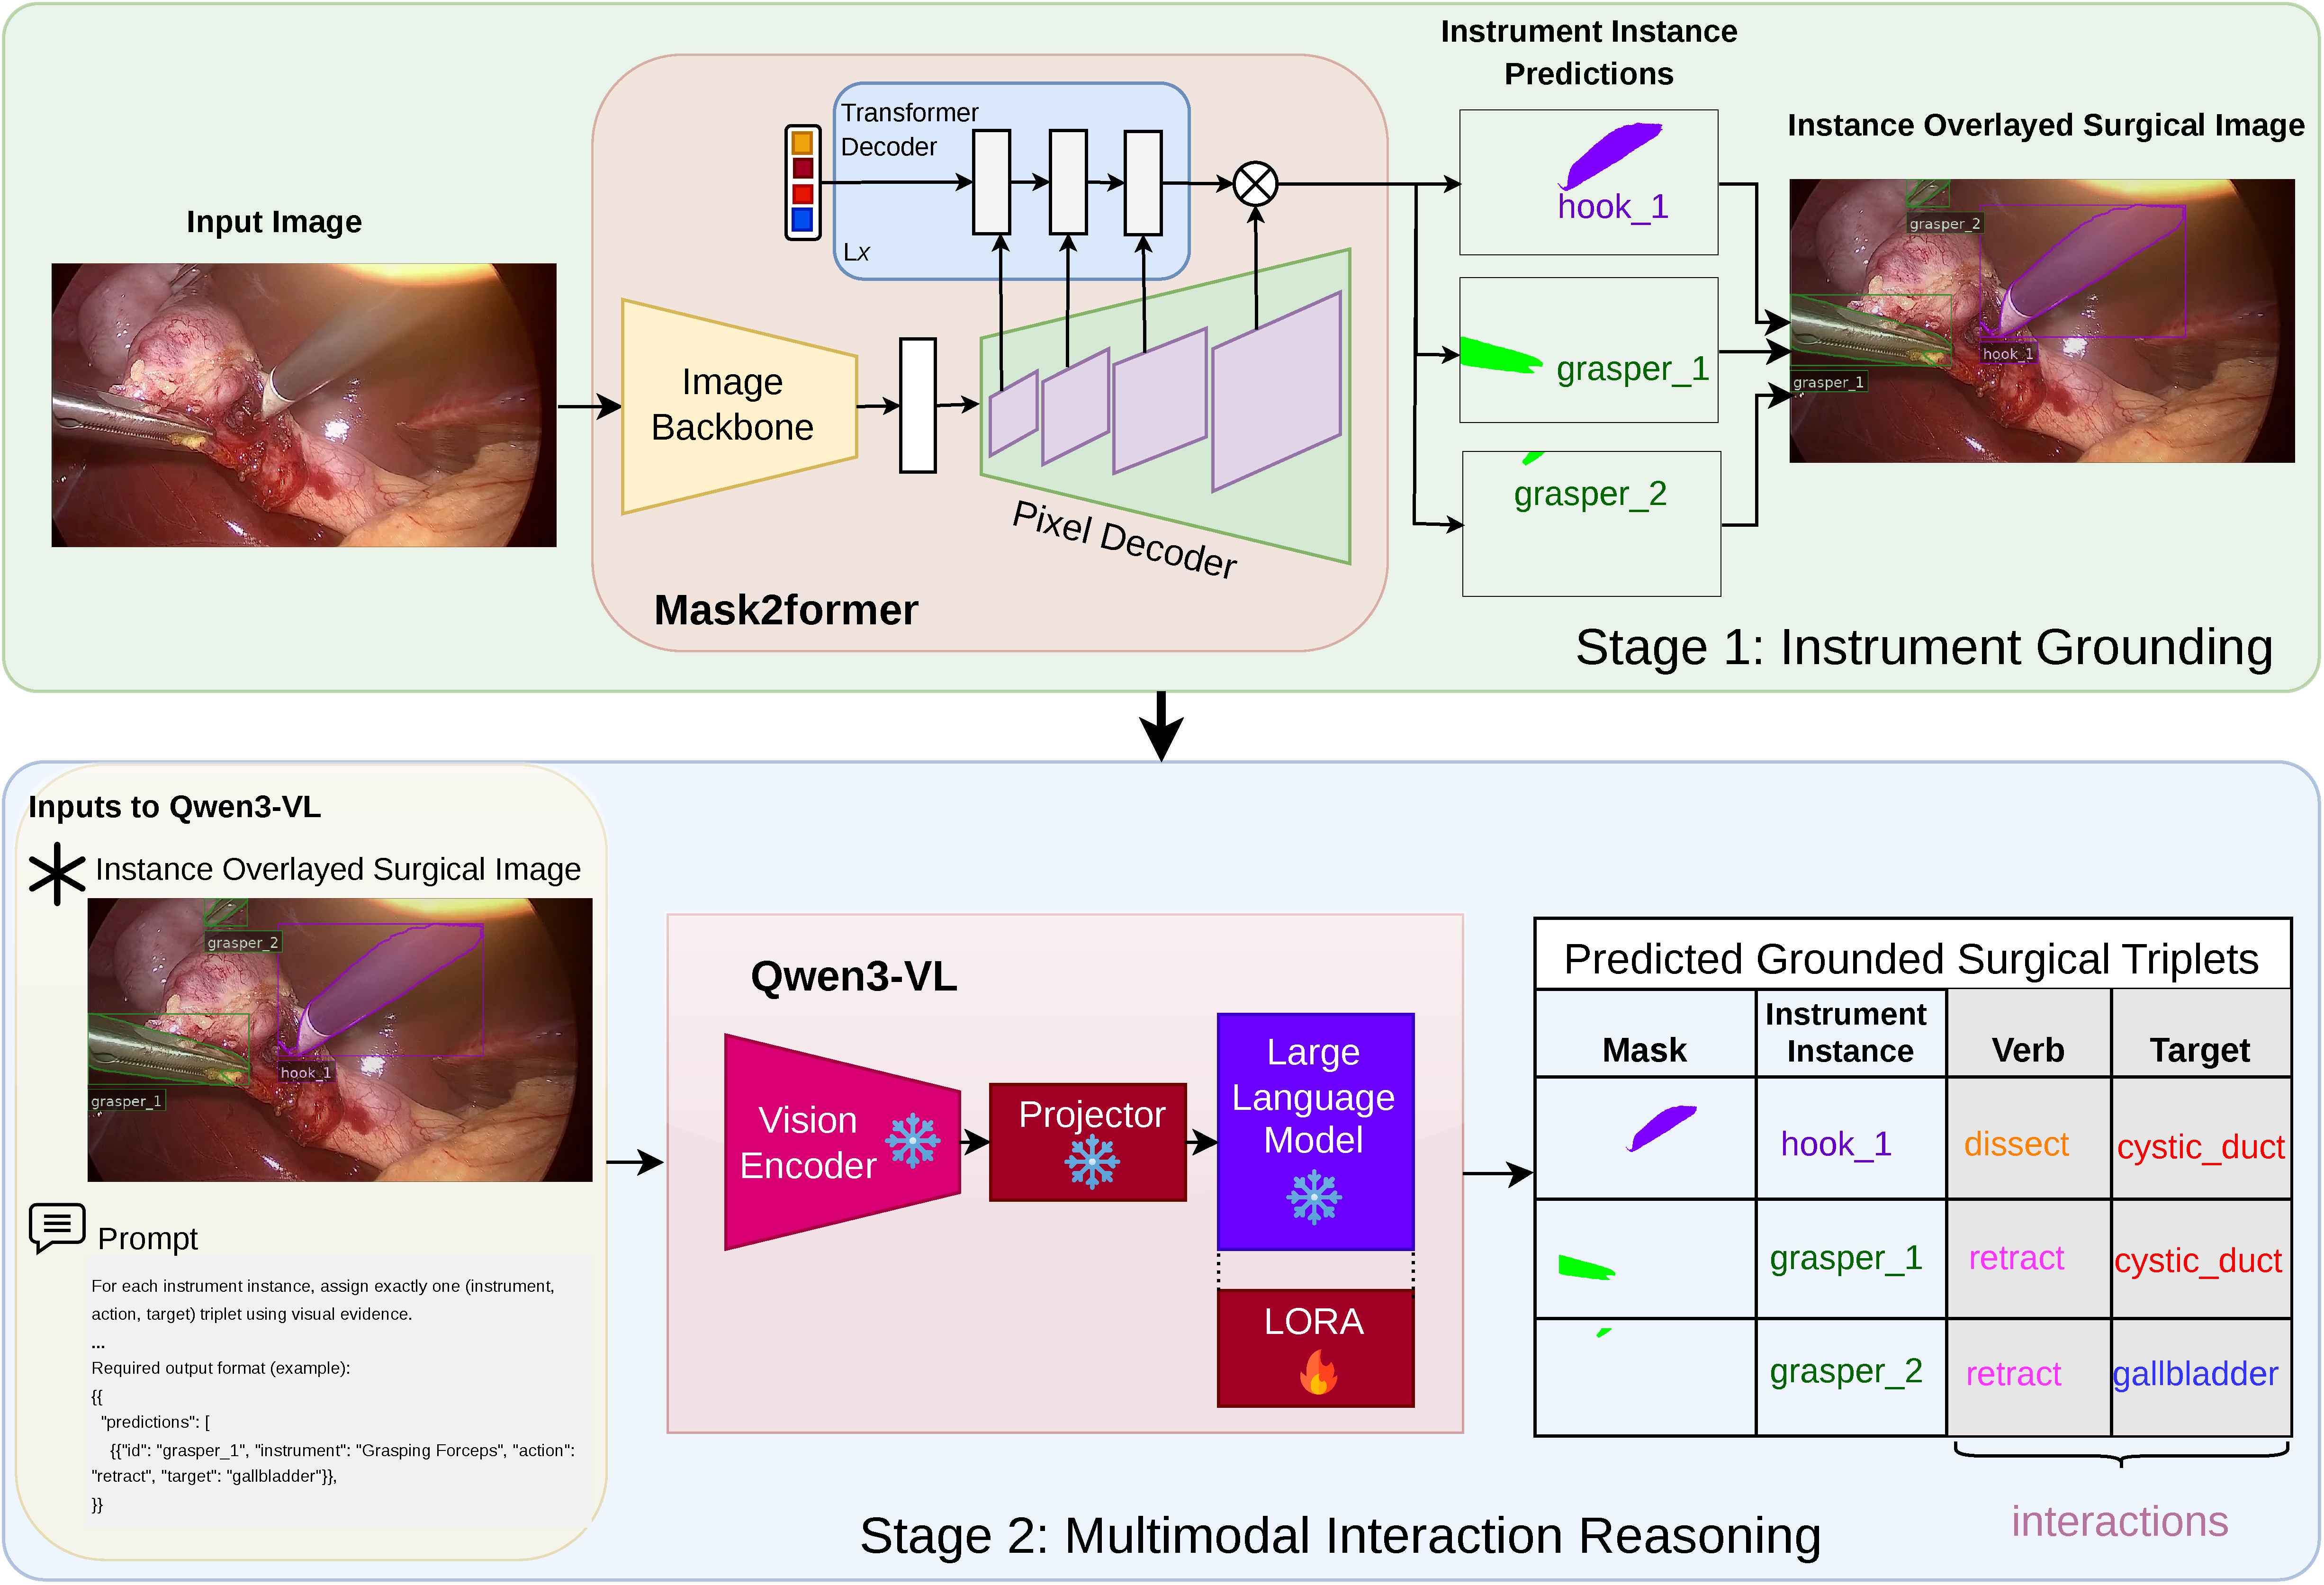
\includegraphics[width=0.95\linewidth]{figures/two_stage_pipeline.pdf}
    \caption{
    Overview of the proposed two-stage surgical triplet segmentation framework.
    In the first stage, Mask2Former localises instrument instances and assigns an instance identifier to each detected instrument. In the second stage, Qwen3-VL performs multimodal interaction reasoning by jointly considering the original image, grounded instrument instances and textual instructions to predict one \ivttriplet interaction for each instrument instance. During supervised fine-tuning, the visual encoder, projector and base language model remain frozen, while only LoRA adapters are optimised.
    }
    \label{fig:framework}
\end{figure}


\subsection{Problem Formulation} \label{sec:problem_formulation}
We formulate surgical triplet segmentation as a two-stage prediction problem consisting of instrument grounding followed by multimodal interaction reasoning. Let $ I \in \mathbb{R}^{H \times W \times 3}$ denote an input laparoscopic image of height $H$ and width $W$. In the first stage, an instance segmentation model detects all visible surgical instruments and produces a set of grounded instrument instances $\mathcal{S} = \{s_i\}_{i=1}^{N},$ where $N$ denotes the number of grounded instrument instances and each grounded instance is represented as $s_i=(m_i,c_i,\mathrm{id}_i).$ Here, $m_i$ denotes the binary segmentation mask, $c_i$ is the instrument category, and $\mathrm{id}_i$ is a unique identifier assigned to distinguish multiple instances belonging to the same instrument class.

Given the grounded instrument set $\mathcal{S}$ and the original image $I$, the
second stage learns the mapping $f_{\theta}(I,\mathcal{S}) \rightarrow \mathcal{Y}$,
where $\mathcal{Y}=\{y_i\}_{i=1}^{N}$ and $y_i=(v_i,t_i)$.
Here, $v_i$ denotes the surgical verb and $t_i$ the corresponding anatomical
target. Throughout this work, we distinguish between experiments performed using ground-truth grounded instrument instances and those using predicted instrument instances from the first-stage grounding model. The former isolates the interaction reasoning stage, whereas the latter evaluates the complete two-stage framework.

The complete surgical triplet associated with instrument instance $i$ is therefore given by $\tau_i=(c_i,v_i,t_i).$ Unlike end-to-end triplet segmentation approaches that jointly optimise localisation and interaction prediction within a single architecture, our formulation explicitly decomposes these tasks. Instrument grounding is performed by a dedicated segmentation model, while multimodal interaction reasoning operates only on grounded instrument instances. This separation allows the interaction prediction stage to remain independent of the underlying grounding architecture and enables improvements to either stage without modifying the other.

\subsection{Multimodal Interaction Reasoning} \label{sec:multimodal_interaction_reasoning}

To realise the interaction prediction function defined in \secref{sec:problem_formulation}, we employ a multimodal large language model (MLLM) that performs multimodal interaction reasoning over grounded instrument instances. Rather than jointly learning localisation and interaction prediction within a single network, the proposed framework assumes that instrument instances have already been grounded and focuses exclusively on predicting the corresponding surgical interactions. An overview of the reasoning stage is illustrated in Figure~\ref{fig:framework}.

\subsubsection{Interaction Reasoning and Structured Prediction}
For each image, the model receives the original RGB image together with coloured mask overlays indicating the grounded instrument instances. Each instance is associated with an instrument category and unique identifier, allowing multiple instances of the same instrument type to be distinguished. A textual instruction specifies the required output format and requests one structured interaction prediction for every grounded instrument instance.

We adopt Qwen3-VL as the interaction reasoning model owing to its strong multimodal understanding and structured generation capabilities. Given the grounded image and textual instruction, the model jointly reasons over the complete surgical scene and predicts one interaction for every grounded instrument instance within a single autoregressive response.

The model generates one structured prediction for each grounded instrument instance consisting of the instance identifier, predicted verb and predicted anatomical target. Generated outputs are parsed into the predefined benchmark format before evaluation. Predictions that cannot be associated with a valid grounded instrument instance are discarded and treated as incorrect.

\subsubsection{Parameter-Efficient Fine-Tuning}
We adopt parameter-efficient fine-tuning using LoRA on the Qwen3-VL-8B model. During training, the vision encoder, multimodal projector and base language model remain frozen, while LoRA adapters are inserted into the language model and optimised using supervised fine-tuning. This substantially reduces the number of trainable parameters while preserving the visual and linguistic knowledge acquired during large-scale pre-training.

\subsection{Investigated Adaptations}

\begin{figure}[htb!]
    \centering
    % Placeholder box (Width, Height)
    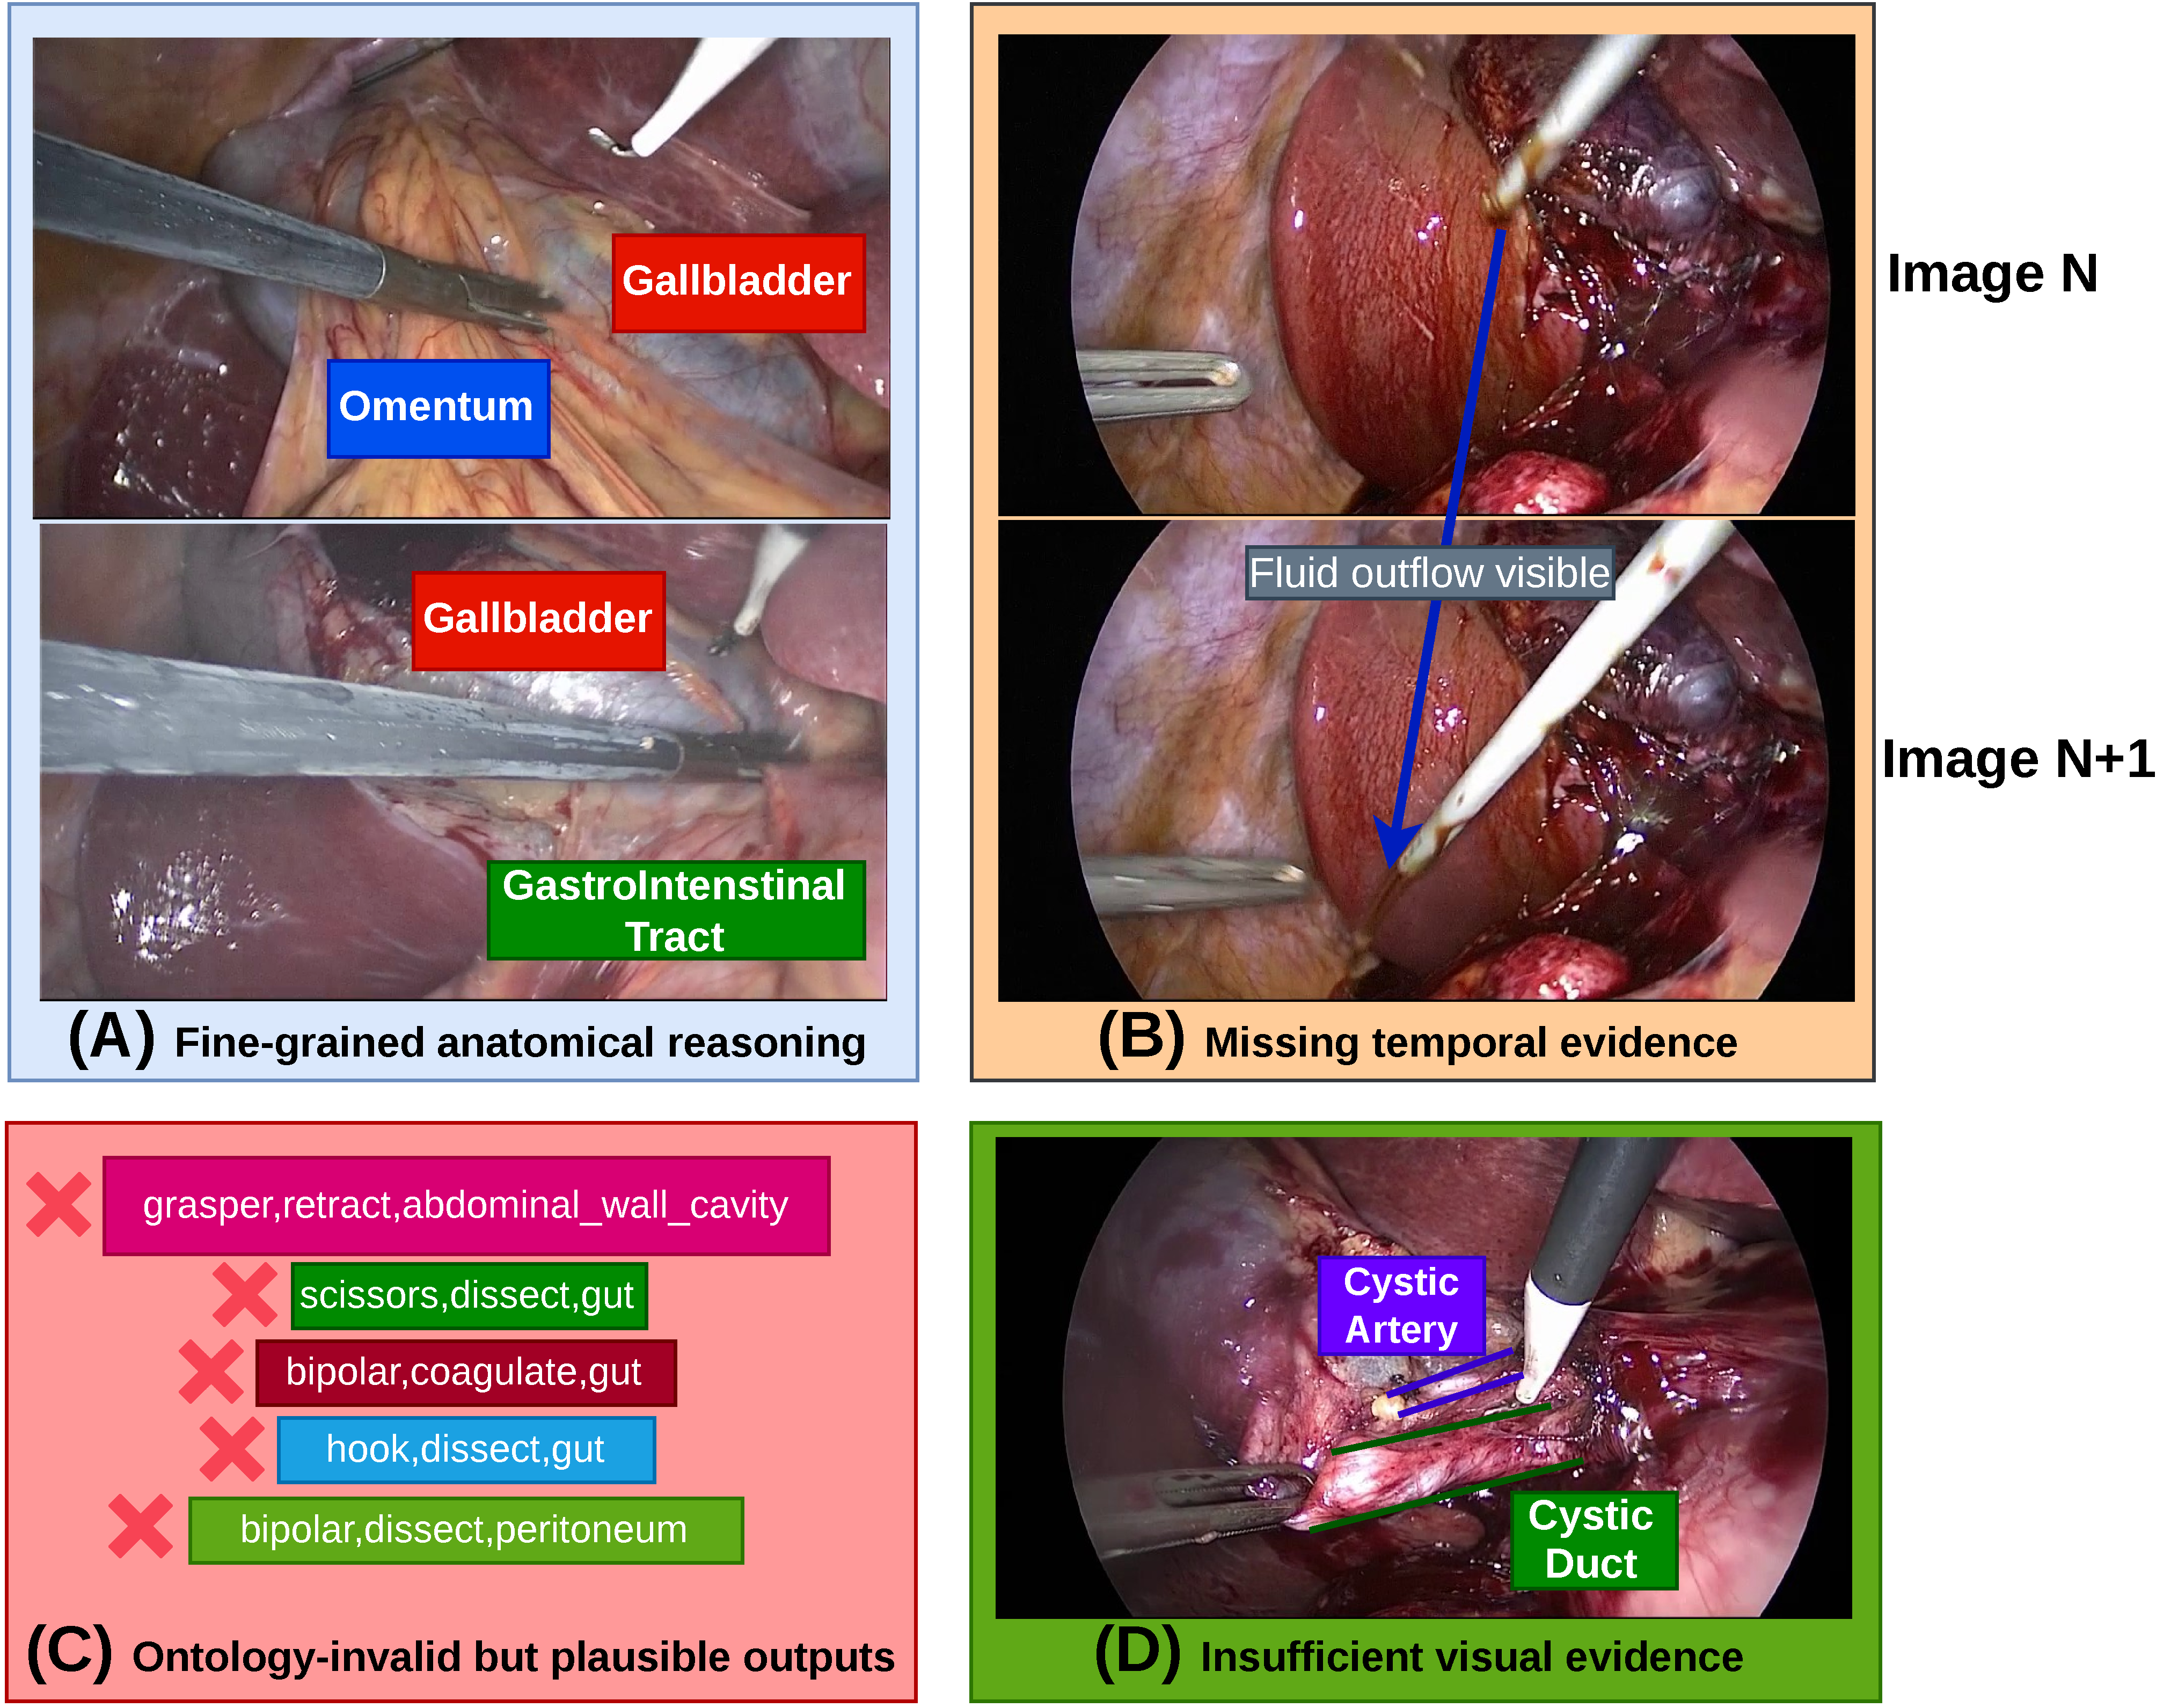
\includegraphics[width=0.95\linewidth]{figures/adaptation_motivation.pdf}
    \caption{
    Representative failure modes motivating the investigated adaptations.
    (A) Fine-grained anatomical ambiguities in which multiple neighbouring tissues
    are visually plausible, but closer analysis of tissue appearance, instrument
    contact and spatial relationships may resolve the interaction.
    (B) Temporal ambiguity, where the current frame does not contain sufficient
    evidence to distinguish interactions such as irrigation and aspiration, while
    the subsequent frame reveals visible fluid flow.
    (C) Semantically plausible instrument--verb--target combinations that fall
    outside the predefined benchmark ontology.
    (D) Some ambiguities cannot be resolved from a single image because the necessary visual evidence is absent. These cases motivate future work incorporating procedural context, anatomy-aware reasoning and longer temporal reasoning.
    }
    \label{fig:adaptation_motivation}
\end{figure}


Although direct supervised fine-tuning provides a strong baseline, error analysis revealed several recurring failure modes that were not fully reflected by aggregate performance metrics. These observations motivated a series of targeted adaptations investigating whether the remaining errors arise from fine-grained anatomical ambiguity, limited temporal information, insufficient reasoning supervision, weak anatomical context, or the unconstrained nature of autoregressive generation. Figure~\ref{fig:adaptation_motivation} summarises the principal motivations.

\subsubsection{Direct Supervised Fine-Tuning}

We first establish a direct supervised fine-tuning baseline in which the multimodal model is trained to autoregressively predict the interaction associated with every grounded instrument instance. The model directly generates the structured output described in Section~3.3 without any intermediate supervision or additional contextual information.

This baseline serves as the reference model for all subsequent investigations and provides insight into the capabilities of autoregressive multimodal interaction prediction under standard supervised fine-tuning.

\subsubsection{Sequential Dialogue Prediction}
The fine-grained anatomical ambiguities illustrated in \figref{fig:adaptation_motivation}(A) suggest that direct joint prediction may require the model to resolve several coupled decisions simultaneously. For example, identifying the anatomical target may depend on first understanding
the type of interaction performed by the instrument. We therefore investigate whether decomposing interaction prediction into simpler, ordered decisions improves multimodal interaction reasoning.

Inspired by divide-and-discern dialogue tuning ~\cite{zhang2026bootstrapping}, which reformulates difficult one-shot prediction as a sequence of progressively simpler dialogue turns, we introduce Sequential Dialogue Prediction. Rather than generating the verb and target jointly, the model first predicts one verb for each grounded instrument instance. In a subsequent dialogue turn, the preceding verb predictions are retained as context and the model predicts the corresponding anatomical targets. The final triplets are constructed by combining the grounded instrument identities with the sequentially generated verbs and targets.

\figref{fig:sequential_dialogue} contrasts this formulation with direct single-turn prediction.

\begin{figure}[htb!]
    \centering
    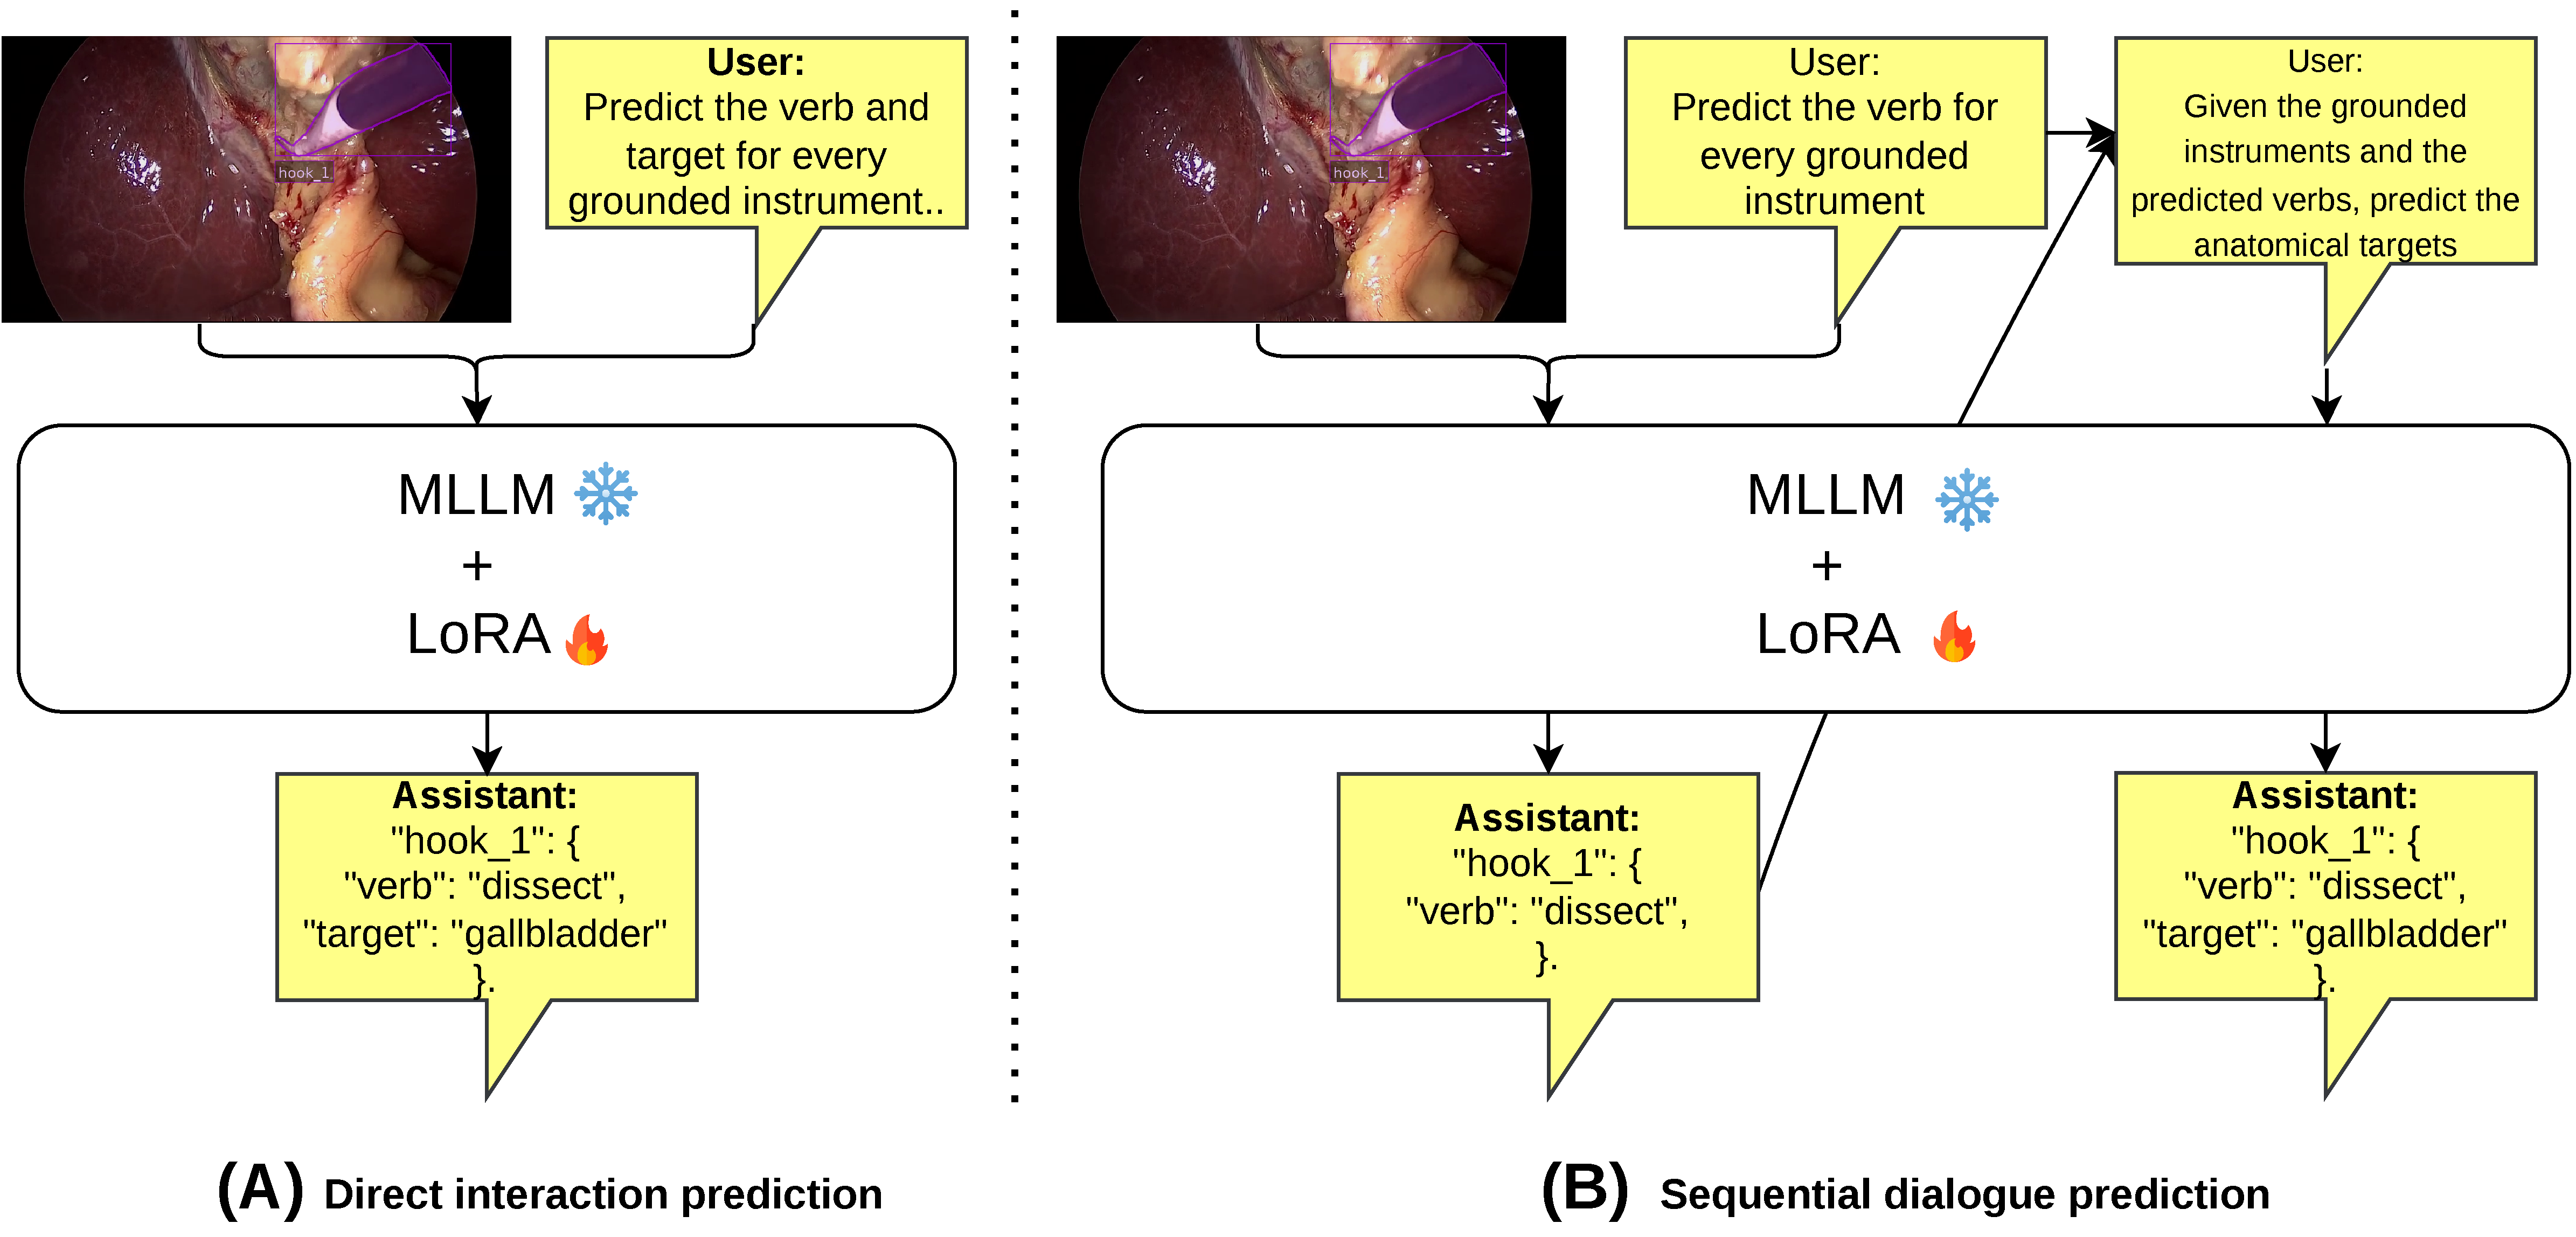
\includegraphics[width=0.95\linewidth]{figures/sequential_dialogue_prediction.pdf}
    \caption{
   Comparison of direct interaction prediction and Sequential Dialogue Prediction. In the direct formulation, the model jointly predicts the verb and anatomical target for each grounded instrument in a single response. In the sequential formulation, the model first predicts the verbs and subsequently predicts the
    targets while retaining the preceding verb predictions as dialogue context.
    The final triplets are constructed by combining the grounded instrument
    identities with the sequentially predicted verbs and targets.
    }
    \label{fig:sequential_dialogue}
\end{figure}


\subsubsection{Temporal Visual Context}

Analysis of difficult prediction cases revealed that several surgical actions and anatomical targets cannot always be determined reliably from a single image. For example, distinguishing between \textit{irrigate} and \textit{aspirate} frequently depends on observing fluid motion across multiple frames, while actions such as \textit{grasp} and \textit{retract} often require temporal evidence describing tissue movement. As illustrated in Figure~\ref{fig:adaptation_motivation}(B), the current frame may not contain sufficient evidence to determine the direction of fluid flow,
whereas the subsequent frame makes the interaction apparent.

Motivated by these observations, we investigate whether incorporating neighbouring video frames improves interaction prediction. Instead of reasoning over an isolated frame, the multimodal model receives a short temporal window centred on the current image, allowing the model to jointly exploit spatial and temporal information when predicting surgical interactions.


\subsubsection{Distilled Reasoning Supervision}
\begin{figure}[htb!]
    \centering
    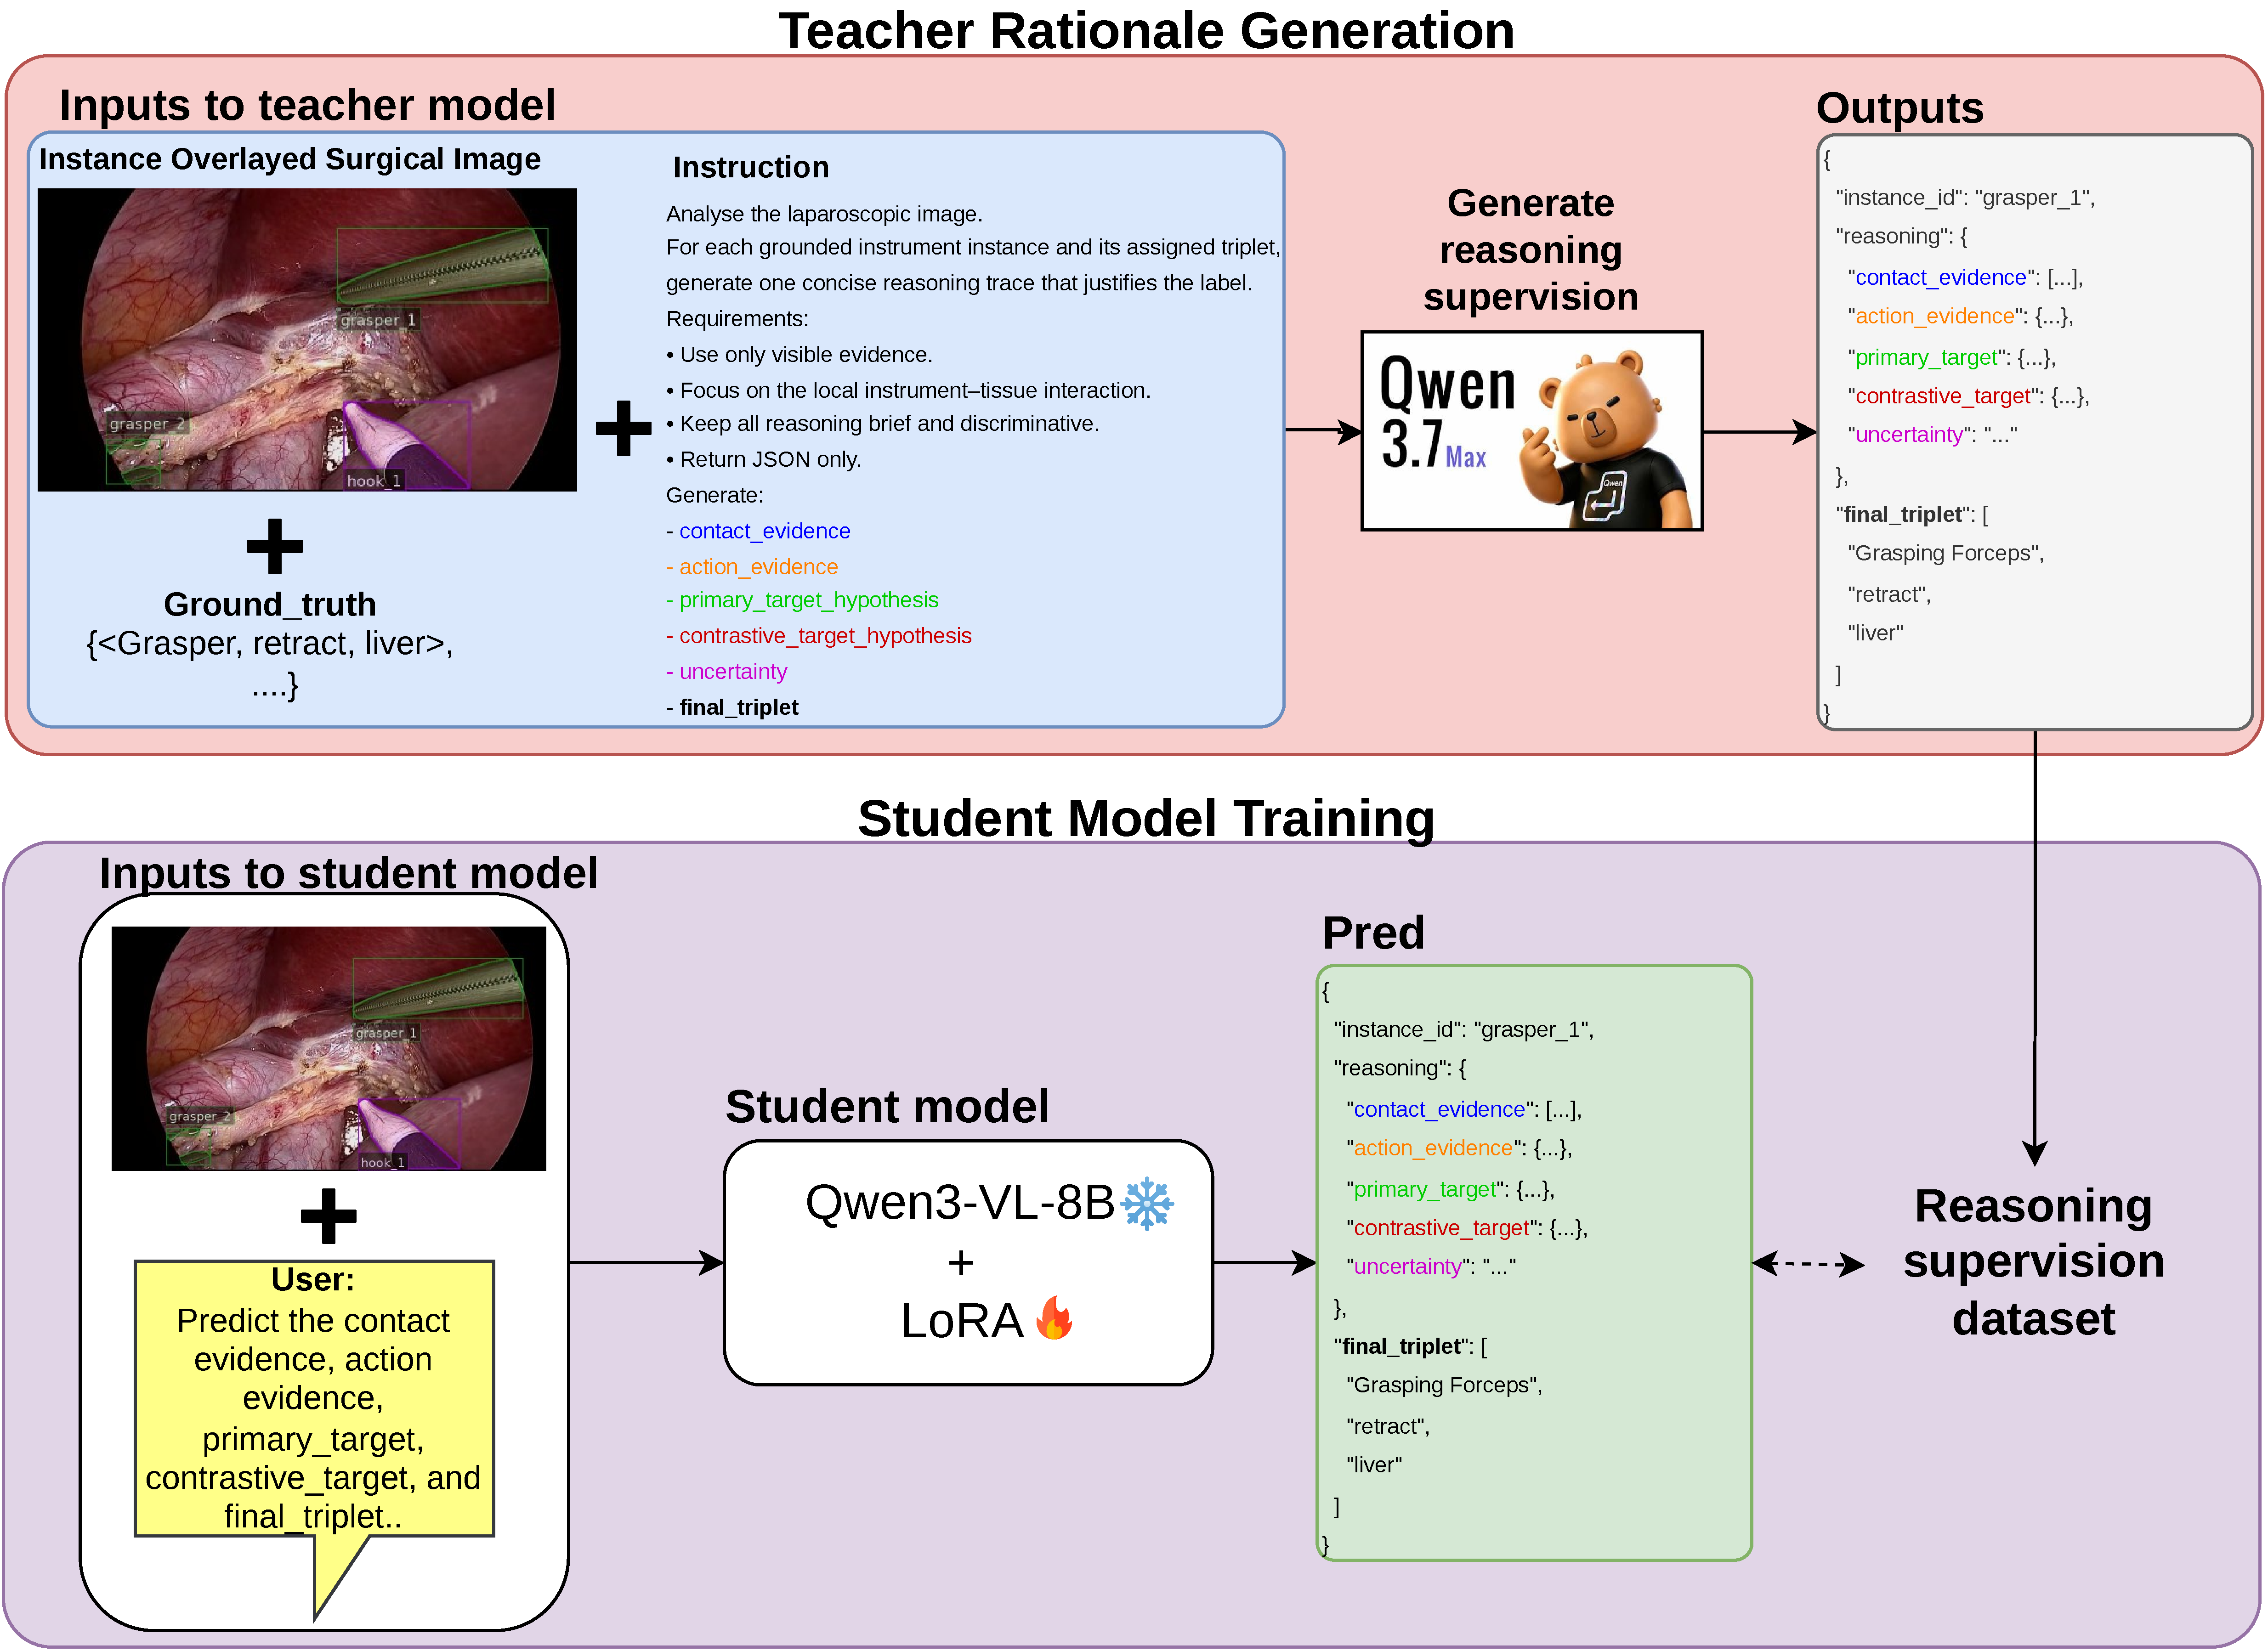
\includegraphics[width=0.95\linewidth]{figures/distilled_reasoning_supervision.pdf}
    \caption{
       Overview of the proposed distilled reasoning supervision pipeline. A stronger teacher MLLM (Qwen3.7-Max) first generates structured reasoning traces for each grounded instrument instance using the image and ground-truth triplet labels as inputs. The generated rationales are collected into a reasoning supervision dataset, which is subsequently used to supervise a smaller student model (Qwen3-VL-8B) during LoRA-based supervised fine-tuning. The student is trained to jointly generate the structured reasoning trace and the final instrument--verb--target triplet.
        }
    \label{fig:distilled_reasoning}
\end{figure}

The fine-grained anatomical ambiguities illustrated in Figure~\ref{fig:adaptation_motivation}(A) suggest that predicting the correct interaction may require more than direct visual recognition. Recent advances in multimodal large language models have shown that explicitly supervising intermediate reasoning can improve performance on complex vision-language tasks. We therefore investigate whether transferring structured reasoning from a stronger teacher model can improve surgical interaction reasoning.

As illustrated in Figure~\ref{fig:distilled_reasoning}, we first use Qwen3.7-Max as a teacher model to generate structured reasoning traces for every grounded instrument instance. The teacher receives the overlaid surgical image together with the corresponding ground-truth \ivttriplet\ label and is prompted to produce a concise rationale consisting of contact evidence, action evidence, a primary target hypothesis, a contrastive target hypothesis, an uncertainty statement, and the final triplet. The generated rationales are collected to form a reasoning supervision dataset.

During supervised fine-tuning, the student model receives only the grounded surgical image and the reasoning prompt. It is trained to jointly generate both the structured reasoning trace and the final \ivttriplet\ prediction. This formulation encourages the model to learn intermediate reasoning representations while retaining direct supervision of the final structured prediction.

\subsubsection{Anatomical Context Priors}
Several target prediction errors occurred between neighbouring anatomical structures with highly similar visual appearance. We hypothesized that providing coarse anatomical context around the instrument tip could reduce this ambiguity.

To investigate this hypothesis, weak anatomical priors obtained from an external anatomy segmentation model are incorporated into the textual prompt as additional contextual information. Rather than providing explicit target labels, these priors supply coarse anatomical evidence surrounding the instrument tip while allowing the multimodal model to perform the final interaction prediction.

\subsubsection{Ontology-Guided Prompting}
The failure mode illustrated in Figure~\ref{fig:adaptation_motivation}(C) shows that autoregressive interaction prediction occasionally produces \ivttriplet combinations that are semantically plausible but do not exist within the predefined surgical interaction ontology. Although these combinations may appear clinically reasonable, they are considered invalid predictions under the benchmark definition.

To investigate whether explicitly providing knowledge of the interaction ontology improves prediction consistency, we include the valid interaction combinations associated with each grounded instrument category as part of the instruction prompt. Rather than modifying the autoregressive decoding process, the ontology is incorporated as additional textual context describing the valid interaction space while allowing the model to freely generate the final prediction.

This formulation represents a lightweight approach to incorporating prior knowledge without introducing architectural modifications or ontology-guided Prompting.



\section{Experimental Setup}

\subsection{Dataset}
Experiments were conducted on the CholecTripletSeg benchmark, a surgical triplet segmentation dataset. Each image contains pixel-level instrument instance annotations together with the corresponding  \ivttriplet interaction labels. Following the evaluation protocol introduced in~\cite{alabi2026grounding}, all experiments use the official training, validation and test splits. Additional details regarding the dataset construction and annotation protocol are provided in~\cite{alabi2026grounding}.

\subsection{Evaluation Protocol}
Performance is evaluated using the official CholecTripletSeg evaluation protocol, which reports mean Average Precision (mAP) for instrument (AP$_I$), verb (AP$_V$), target (AP$_T$), \ivpair (AP$_{IV}$), \itpair (AP$_{IT}$), and complete \ivttriplet triplets (AP$_{IVT}$).

To separately evaluate the proposed interaction reasoning stage and the complete two-stage framework, experiments are conducted under two evaluation settings.

The first assumes ground-truth instrument grounding, where manually annotated instrument instances are provided to the interaction reasoning model. This setting isolates the interaction prediction task from localisation errors and enables direct evaluation of the reasoning stage.

The second uses predicted instrument instances generated by A standard first-stage Mask2Former model. This setting evaluates the complete two-stage pipeline under realistic deployment conditions and captures the influence of grounding errors on overall triplet prediction performance.

\subsection{Implementation Details}
All multimodal interaction reasoning models were based on \textbf{Qwen3-VL-8B-Instruct}. We used Low-Rank Adaptation (LoRA) for parameter-efficient supervised fine-tuning. The vision encoder, multimodal projector and base language model remain frozen throughout training, and only the LoRA parameters inserted into the language model were optimised. Unless otherwise stated, LoRA rank was set to $r=64$, with scaling factor $\alpha=128$ and dropout $0.05$.

Models were trained using fused AdamW with an initial learning rate of $2\times10^{-4}$, weight decay of $0.01$, a warm-up ratio of $0.03$, and gradient clipping with a maximum norm of $1.0$. The per-device training and validation batch sizes were both set to one. Gradients were accumulated over 32 steps, yielding an effective batch size of 32 samples. Training was performed for five epochs with random seed 42. FlashAttention-2 was used for efficient attention computation.

For single-frame experiments, including direct supervised fine-tuning, sequential dialogue prediction, distilled reasoning supervision, anatomical context priors, and ontology-guided Prompting, images were processed using a minimum visual token budget corresponding to $256\times28\times28$ pixels and a maximum budget of $768\times28\times28$ pixels.

The temporal experiments followed the same optimisation and LoRA configuration. For the cached three-frame experiment, the training configuration was unchanged from the single-frame baseline. For the native multi-frame implementation, the per-frame visual budget was reduced to a minimum of $64\times64$ pixels and a maximum of $256\times256$ pixels to control the memory and computational cost introduced by multiple frames.

Validation was performed periodically during training. Single-frame experiments were generally evaluated every $5\%$ of the total optimisation steps, while the native video implementation used validation once per epoch. Early stopping was applied using validation loss, with patience set to six evaluations for single-frame experiments and five evaluations for the native video models. Up to ten checkpoints were retained.

For all experiments we ensured to keep the optimization parameters as simialr as possible, because we observed differences with batch size, learning rate and duration of training. 

\subsection{Compared Methods}
We compare the proposed interaction reasoning framework against representative approaches for surgical triplet prediction.

\begin{itemize}
\item Rendezvous (RDV), a weakly supervised frame-level triplet recognition model, adapted for triplet segmentation

\item Mask2Former Triplet Segmentation, the baseline one-stage grounded triplet segmentation model introduced in CholecTripletSeg.

\item TargetFusionNet, which incorporates weak anatomical priors within a Mask2Former-based grounded triplet segmentation architecture.

\item The investigated multimodal interaction reasoning models presented in this work.
\end{itemize}

\section{Results}
\subsection{Interaction Prediction under Ground-Truth Grounding}
We first evaluate the multimodal interaction reasoning stage using ground-truth instrument instances. This controlled setting removes errors introduced by the instrument grounding model and isolates the ability of the MLLM to predict the verb and anatomical target associated with each instrument instance. Since the instrument category is provided as input, AP$_I$ is fixed at 100 and is omitted
from Table~\ref{tab:gt_grounding_results}.

\begin{table*}[t]
\centering
\caption{Interaction prediction performance under ground-truth instrument
grounding. All methods receive the ground-truth instrument instances and
categories. The best result in each column is shown in bold.}
\label{tab:gt_grounding_results}
\begin{tabular}{lccccc}
\toprule
Method
& AP$_V$
& AP$_T$
& AP$_{IV}$
& AP$_{IT}$
& AP$_{IVT}$ \\
\midrule
Direct SFT
& 55.99 & \textbf{26.35} & 31.03 & 21.87 & 14.56 \\

Sequential dialogue prediction
& 55.92 & 26.21 & 30.48 & 21.61 & 15.31 \\

Anatomical context prior
& 53.35 & 26.27 & 31.48 & \textbf{23.15} & 14.96 \\

Temporal visual context, 3 frames
& \textbf{56.31} & 26.32 & \textbf{32.37} & 21.66 & \textbf{15.89} \\

Temporal visual context, 5 frames
& 53.52 & 22.10 & 27.72 & 17.39 & 11.61 \\

Distilled Reasoning Supervision
& 53.22 & 20.88 & 27.30 & 13.59 & 8.69 \\
\bottomrule
\end{tabular}
\end{table*}

Direct supervised fine-tuning provides a strong baseline, achieving an
AP$_{IVT}$ of 14.56. Among the investigated adaptations, temporal
context yields the strongest complete-triplet performance, increasing
AP$_{IVT}$ to 15.89. It also obtains the highest verb and instrument--verb
performance, suggesting that neighbouring frames provide useful evidence for
distinguishing actions whose interpretation depends on motion or temporal
progression.

sequential dialogue prediction also improves complete-triplet performance,
reaching an AP$_{IVT}$ of 15.31, although it does not improve the individual
verb or target metrics. This suggests that conditioning target prediction on the previously predicted verb may improve complete-triplet consistency of the complete
interaction without uniformly improving each component.

The anatomical tip prior produces a smaller increase in AP$_{IVT}$, from 14.56
to 14.96, and obtains the highest AP$_{IT}$ among the directly comparable
five-epoch variants. However, the improvement is not reflected in AP$_T$,
suggesting that the additional anatomical evidence changes the association
between instruments and targets without consistently improving target
classification in isolation.

Longer temporal context does not provide further gains. The five-frame model
substantially underperforms both the three-frame model and the single-frame
baseline. This suggests that simply increasing the number of input frames is
insufficient and may introduce irrelevant visual information or increase the
difficulty of optimisation.

Explicit reasoning supervision also fails to consistently improve aggregate
performance. Multitask reasoning supervision obtains strong AP$_{IV}$ and
AP$_{IT}$ values but does not improve complete-triplet AP. Training exclusively
on generated reasoning traces performs substantially worse, particularly for
target-related metrics. These results suggest that long generated rationales
may dilute supervision of the final structured prediction when all generated
tokens are optimised equally.


\subsection{Complete Two-Stage Triplet Segmentation}

We next evaluate the complete pipeline using instrument instances predicted by
the first-stage Mask2Former model. Unlike the ground-truth-grounding evaluation,
this setting includes both localisation and interaction prediction errors and
therefore reflects the practical performance of the two-stage framework.

\begin{table*}[t]
\centering
\caption{Performance of the complete two-stage framework using predicted
instrument instances. The previously published one-stage triplet segmentation
model is included as a reference.}
\label{tab:predicted_grounding_results}
\begin{tabular}{lcccccc}
\toprule
Method
& AP$_I$
& AP$_V$
& AP$_T$
& AP$_{IV}$
& AP$_{IT}$
& AP$_{IVT}$ \\
\midrule

RDV-Det \cite{nwoye2023cholectriplet2022} 
&0.09 &0.11 &0.08 &0.08 &0.04 &0.03 \\

Mask2Former-Triplet \cite{alabi2026grounding} 
&65.24 &45.61 &20.75 &23.03 &16.47 &12.23 \\

TargetFusionNet \cite{alabi2026grounding}
& 67.19 & 46.23 & 23.70 & 24.82 & 17.74 & 13.45 \\

Two-stage Direct SFT
& \textbf{80.64} & \textbf{51.89} & \textbf{25.27}
& \textbf{29.01} & \textbf{18.73} & \textbf{13.52} \\

\bottomrule
\end{tabular}
\end{table*}

Using predicted instrument instances reduces performance relative to the
ground-truth-grounding setting, as errors from the first stage propagate into
the interaction prediction stage. Nevertheless, the two-stage Direct SFT model
achieves an AP$_I$ of 80.64, substantially higher than the previously reported
one-stage model, while improving AP$_V$, AP$_T$, AP$_{IV}$ and AP$_{IT}$.
Complete-triplet performance is comparable, increasing slightly from 13.45 to
13.52 AP$_{IVT}$.

The relatively small improvement in AP$_{IVT}$ despite stronger component-level
performance demonstrates the difficulty of complete triplet prediction: an
output is correct only when the instrument, verb and target are all predicted
correctly and associated with the same instance. Errors from either stage
therefore compound at the full-triplet level.


\subsection{Influence of Optimisation}
During model development, we observed that changes in optimisation strategy often
produced performance differences comparable to those obtained through the
investigated reasoning adaptations. To provide context for interpreting the
subsequent experiments, we report a small exploratory study examining the
influence of training duration, effective batch size and learning rate under
ground-truth instrument grounding.

These experiments are not intended as methodological contributions or a
comprehensive hyperparameter search. Rather, they demonstrate that optimisation
choices can substantially influence interaction prediction performance and
should therefore be considered when comparing different adaptation strategies. They take the direct interaction prediction method and change parameters. 


\begin{table*}[t]
\centering
\caption{Influence of optimisation settings on direct supervised fine-tuning under ground-truth instrument grounding. All experiments use the same model architecture and differ only in optimisation hyperparameters.}
\label{tab:optimisation_results}
\begin{tabular}{lccc|ccccc}
\toprule
Method & Effective Batch & Epochs & LR
& AP$_V$ & AP$_T$ & AP$_{IV}$ & AP$_{IT}$ & AP$_{IVT}$ \\
\midrule
Direct SFT (baseline)        & 32  & 5  & $2\times10^{-4}$ & 55.99 & 26.35 & 31.03 & 21.87 & 14.56 \\

Direct SFT                   & 8   & 10 & $2\times10^{-4}$ & \textbf{58.57} & \textbf{28.45} & \textbf{33.28} & 20.61 & 15.04 \\

Direct SFT                   & 128 & 10 & $2\times10^{-5}$ & 55.51 & 28.18 & 30.41 & 20.35 & 14.78 \\

Direct SFT                   & 48  & 20 & $2\times10^{-5}$ & 56.49 & 26.82 & 33.10 & 21.50 & 15.68 \\

Direct SFT                   & 64  & 30 & $2\times10^{-5}$ & 53.86 & 26.68 & 32.24 & \textbf{23.21} & \textbf{16.05} \\


\bottomrule
\end{tabular}
\end{table*}

The results in Table~\ref{tab:optimisation_results} demonstrate that optimisation choices can substantially influence interaction prediction performance. Increasing the effective batch size and extending the training duration did not produce uniform improvements across all evaluation metrics. While longer training with larger effective batch sizes generally improved AP$_{IT}$ and AP$_{IVT}$, performance on the individual verb, target and instrument-verb metrics did not consistently improve and, in some cases, deteriorated relative to the baseline. Conversely, the smaller effective batch size of 8 achieved the highest AP$_V$, AP$_T$ and AP$_{IV}$ despite using the original learning rate.

Overall, these experiments indicate that optimisation alone can produce performance differences comparable to several of the investigated interaction reasoning adaptations. They also suggest that different components of the interaction prediction task may favour different optimisation regimes, motivating a more comprehensive optimisation study in future work. Because multiple optimisation variables differ between runs, these results characterise overall sensitivity but do not isolate the contribution of any single hyperparameter


\section{Discussion}
\subsection{Why does direct supervised fine-tuning work so well?}

One of the most surprising findings of this work is the strong performance of direct supervised fine-tuning. Despite the increasing popularity of explicit reasoning supervision, auxiliary anatomical information and increasingly sophisticated prompting strategies, a relatively simple autoregressive formulation provides a competitive baseline for interaction prediction.

We believe this result is largely a consequence of the proposed two-stage formulation. By separating instrument grounding from interaction prediction, the multimodal model is no longer required to solve dense localisation and semantic reasoning simultaneously. Instead, the model receives grounded instrument instances together with the surrounding visual context and can focus exclusively on predicting the associated interaction. This decomposition substantially simplifies the prediction problem and allows the pretrained multimodal model to exploit its existing visual and linguistic knowledge.

These observations suggest that, for grounded surgical interaction prediction, careful problem formulation may be more important than increasingly complex architectural modifications. Rather than introducing additional reasoning mechanisms, establishing a strong supervised fine-tuning baseline should be considered an essential first step when adapting multimodal foundation models to surgical scene understanding.

\subsection{Understanding the Investigated Adaptations}

The investigated adaptations reveal several useful insights into the behaviour of multimodal large language models for surgical interaction prediction.

Among the investigated methods, short-range temporal context consistently produced the largest improvement in complete triplet prediction. This finding is intuitive, as many surgical actions are inherently dynamic. Distinguishing between interactions such as \textit{grasp} and \textit{retract}, or \textit{irrigate} and \textit{aspirate}, often requires observing instrument motion rather than analysing a single static frame. In contrast, extending the temporal window further did not provide additional gains, suggesting that naïvely increasing temporal context is insufficient without explicitly modelling temporal dependencies.

sequential dialogue prediction also provided consistent improvements over direct joint prediction. Predicting the surgical verb before the anatomical target reduces the complexity of the prediction task and provides additional semantic context that can guide subsequent target prediction.

In contrast, several intuitively appealing adaptations did not consistently improve performance. Distilled reasoning supervision produced only marginal gains, while reasoning-only supervision substantially degraded target prediction. Similarly, weak anatomical context priors and ontology-guided Prompting failed to produce reliable improvements across the evaluated metrics. These observations suggest that simply providing additional information does not guarantee better interaction prediction. Instead, future work may require more effective mechanisms for integrating anatomical knowledge and reasoning supervision into multimodal foundation models.

\subsection{Limitations}

This work has several limitations.

First, most investigated adaptations were evaluated using ground-truth instrument instances. This design was intentional, allowing the interaction prediction stage to be studied independently of localisation errors. Although experiments using predicted instrument instances demonstrate that the proposed approach transfers to a practical two-stage pipeline, additional evaluation of all investigated adaptations under predicted grounding remains future work.

Second, several promising ideas could not be fully explored because of computational constraints. In particular, the temporal models, optimisation studies and several adaptation strategies were only partially investigated. Consequently, the results presented in this work should be viewed as an exploration of the proposed design space rather than an exhaustive evaluation.

Finally, all experiments were conducted on CholecTripletSeg. Although this benchmark provides the first large-scale instance-grounded surgical triplet segmentation dataset, evaluating the proposed framework across additional procedures and surgical domains will be necessary to assess its broader generalisation.

Furthermore, the investigated adaptations were evaluated primarily in isolation;
their compatibility and potential cumulative effects were not examined.

\subsection{Future Directions}

The findings of this work suggest that future progress is likely to arise from combining complementary interaction reasoning strategies rather than developing increasingly complex individual adaptations. Although each investigated modification was evaluated independently in order to better understand its contribution, many of these approaches address different sources of ambiguity and are therefore expected to complement one another within a unified interaction reasoning framework.

The encouraging performance of short-range temporal context suggests that future systems should explicitly model procedural continuity rather than treating neighbouring frames as additional visual inputs. Integrating temporal reasoning with interaction reasoning could allow models to exploit instrument motion, tissue deformation and procedural progression to resolve ambiguities that cannot be inferred from a single frame.

Another promising direction is comparison-based interaction reasoning. Instead of relying solely on parametric knowledge, future models could retrieve visually or semantically similar surgical interactions from a reference database and reason by comparison. Such retrieval mechanisms may provide stronger evidence for distinguishing anatomically similar structures or rare interactions than direct prediction alone. Similarly, future training objectives could incorporate auxiliary contrastive tasks in which the model is presented with highly similar interaction pairs and required to explain or identify the subtle differences between them. We believe such comparison-based supervision may encourage finer-grained anatomical understanding than independent interaction prediction alone.

The distilled reasoning supervision experiments also highlight opportunities for improving reasoning supervision itself. Rather than relying solely on automatically generated rationales, future work could investigate expert-reviewed reasoning traces, iterative teacher refinement, or multi-agent verification frameworks to improve the quality of the distilled supervision before fine-tuning.

Similarly, ontology-guided prompting represents only a lightweight mechanism for incorporating prior surgical knowledge. Future work could instead integrate the surgical interaction ontology directly into the decoding process by hierarchically constraining the prediction space or masking invalid \ivttriplet combinations during autoregressive decoding. Such approaches would ensure structurally valid predictions while preserving the flexibility of language-model-based interaction reasoning.

Finally, the proposed framework should be evaluated beyond laparoscopic cholecystectomy. Recent datasets, such as ProstaTD, extend grounded surgical triplet understanding to robot-assisted prostatectomy and provide an opportunity to assess whether the proposed interaction reasoning strategies generalise across surgical procedures. We believe demonstrating such cross-procedure generalisation will be an important step towards more broadly applicable surgical foundation models.

\section{Conclusion}
In this work, we investigated multimodal large language models for interaction prediction within a two-stage surgical triplet segmentation framework. By separating instrument grounding from multimodal interaction reasoning, we formulated surgical triplet segmentation as two complementary problems and established a strong autoregressive supervised fine-tuning baseline for the interaction prediction stage.

Through a series of investigated adaptations, we examined the influence of temporal context, sequential dialogue prediction, distilled reasoning supervision, anatomical context priors and ontology-guided Prompting. Our results demonstrate that direct supervised fine-tuning provides a surprisingly strong baseline, while short-range temporal context and sequential dialogue prediction produce the most consistent improvements. In contrast, several more sophisticated adaptations, including reasoning supervision and anatomical context priors, do not consistently improve interaction prediction.

More broadly, this work highlights the importance of careful problem formulation when adapting multimodal foundation models to structured surgical scene understanding. Together, the proposed formulation and empirical observations provide a foundation for future work on multimodal interaction reasoning and grounded
surgical scene understanding.


\bibliographystyle{splncs04}
\bibliography{mybibliography}
\end{document}